\section{Light sources}
In gpvdm light comes from light sources, which are defined in the light source editor which can be found in the Optical ribbon of the main window see figure \ref{fig:opticalribbon}.

\begin{figure}[H]
\centering
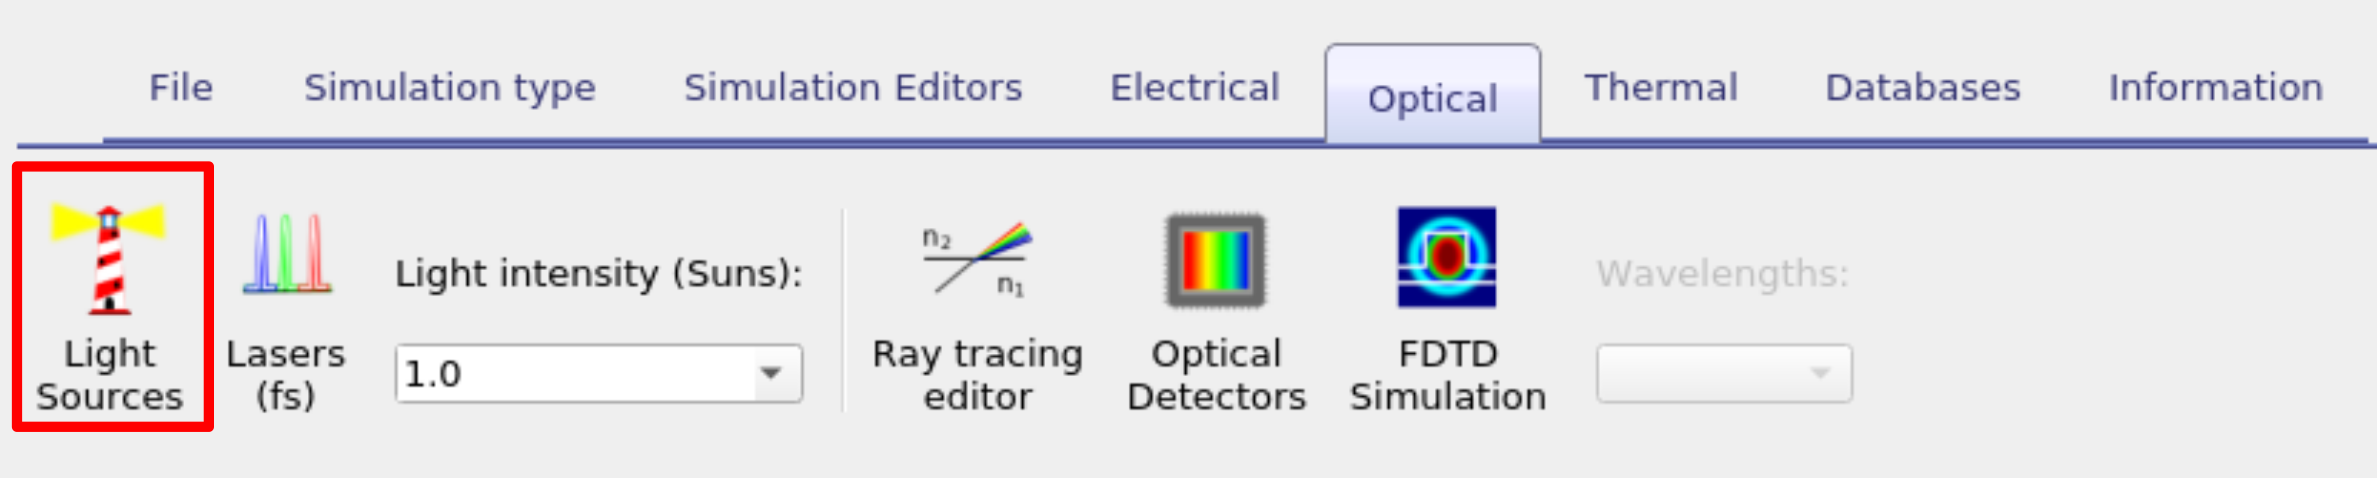
\includegraphics[width=0.7\textwidth]{./images/light_ribbon.png}
\caption{Opening the light source editor.}
\label{fig:opticalribbon}
\end{figure}

The light source editor is shown below in figure \ref{fig:lightsourceeditor}. Each light source consists of of illumination spectra and optical filters. In this way you can define a light source to emit AM1.5G but then filter out various components of the spectrum.  This enables one to simulate for example a device under AM1.5G spectra but behind a thick glass contact which takes sunlight below 300 nm. Light sources can be combined in the "Light source" tab, so for example one could combine AM1.5G and light given off by a fluorescent tube. Each spectrum is multiplied by a "Multiplayer" defined in the "Multiplayer" column this defines the relative intensity of the light sources.

In the filters tab you can define the optical filters. They can be enabled or disabled using the Enable switch, you can select the material which will act as a filter, and decide how much the filter attenuates in dB.

The configure tab of each filter can be used to select where the light comes from, options are:

\begin{enumerate}
  \item Top: Light will come form the top of the device. (y0) This is usually used with the transfer matrix solver. See the bottom left of figure \ref{fig:lightcomesfrom}.
  \item Bottom: Light will come from the bottom of the device. (y1)  This is usually used with the transfer matrix solver.  See the bottom right of figure \ref{fig:lightcomesfrom}.
  \item xyz: The light can come from an xyz position in the simulation space this used for FDTD simulations or ray tracing simulations.  This can be seen in to bottom right of figure \ref{fig:lightcomesfrom}.
\end{enumerate}

Stop and start wavelengths can also be set in the configure tab.

\subsection{Local ground view factor}
The local ground view factor which is given as \cite{neryterrain}

\begin{equation}
F_{ground}=sin^2 \left ( \frac{\theta_t}{2}\right )=\frac{1-cos(\theta_t)}{2}
\end{equation}

can be set in the configure tab.

\begin{figure}[H]
\centering
\begin{tabular}{ c c }

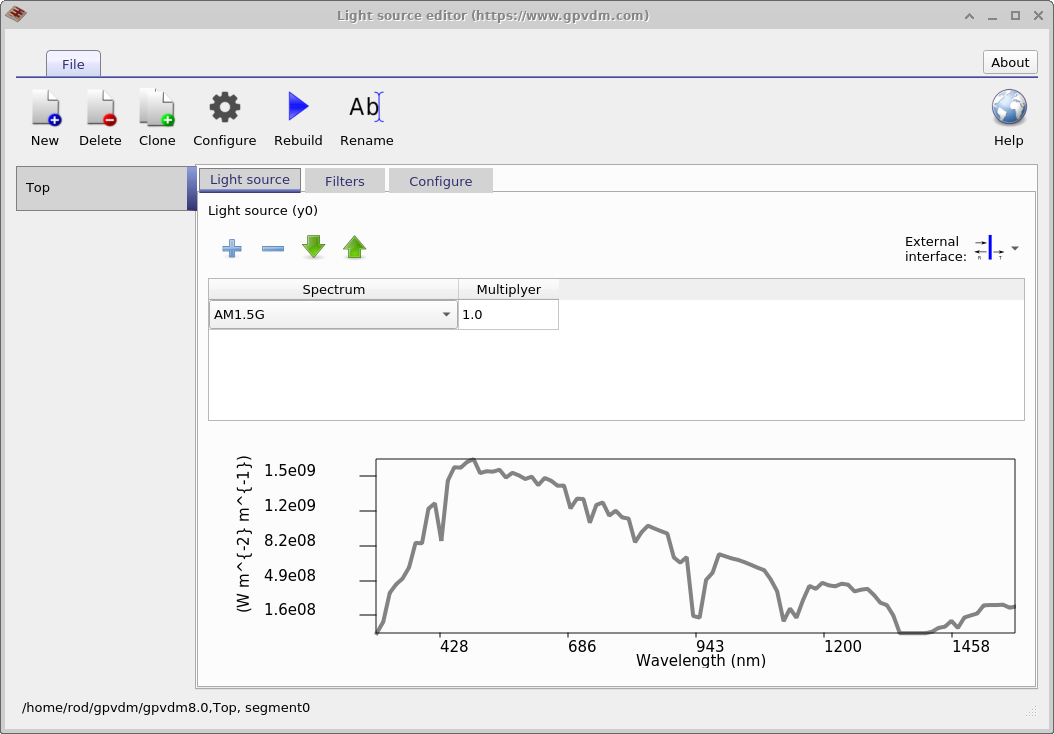
\includegraphics[width=0.5\textwidth,height=0.4\textwidth]{./images/lights0.png}

&
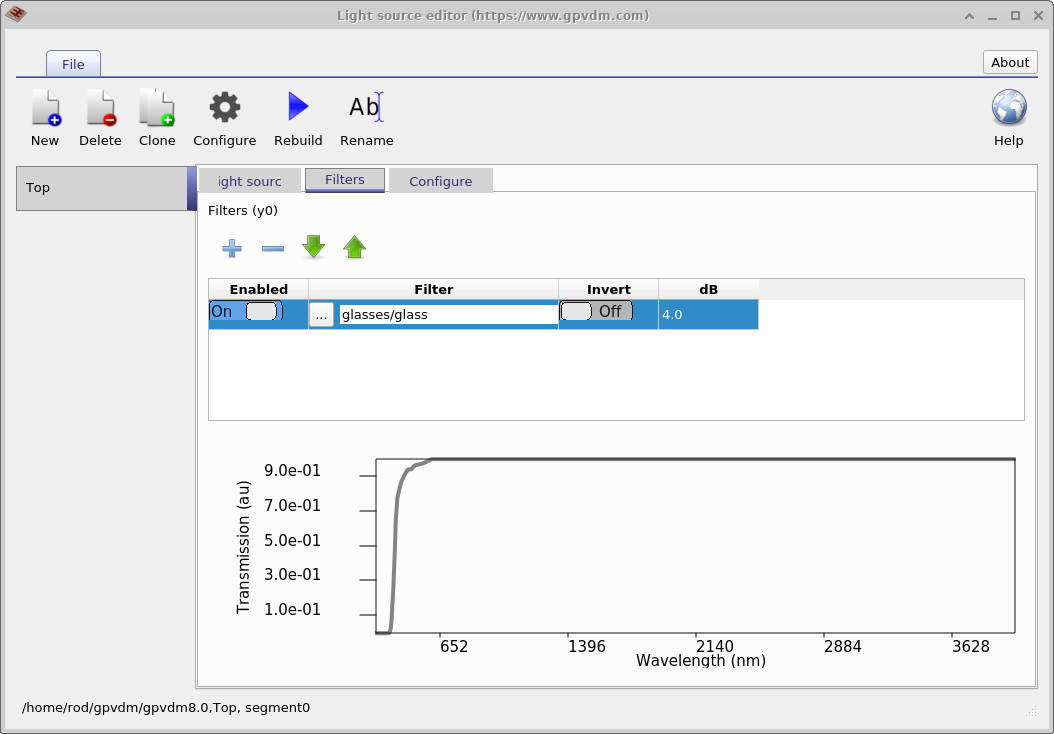
\includegraphics[width=0.5\textwidth,height=0.4\textwidth]{./images/lights1.png}
\\
\end{tabular}
\caption{Left: Building an optical spectrum; Right modifying the light sources with optical filters.}
\end{figure}


\begin{figure}[H]
\centering
\begin{tabular}{ c c }

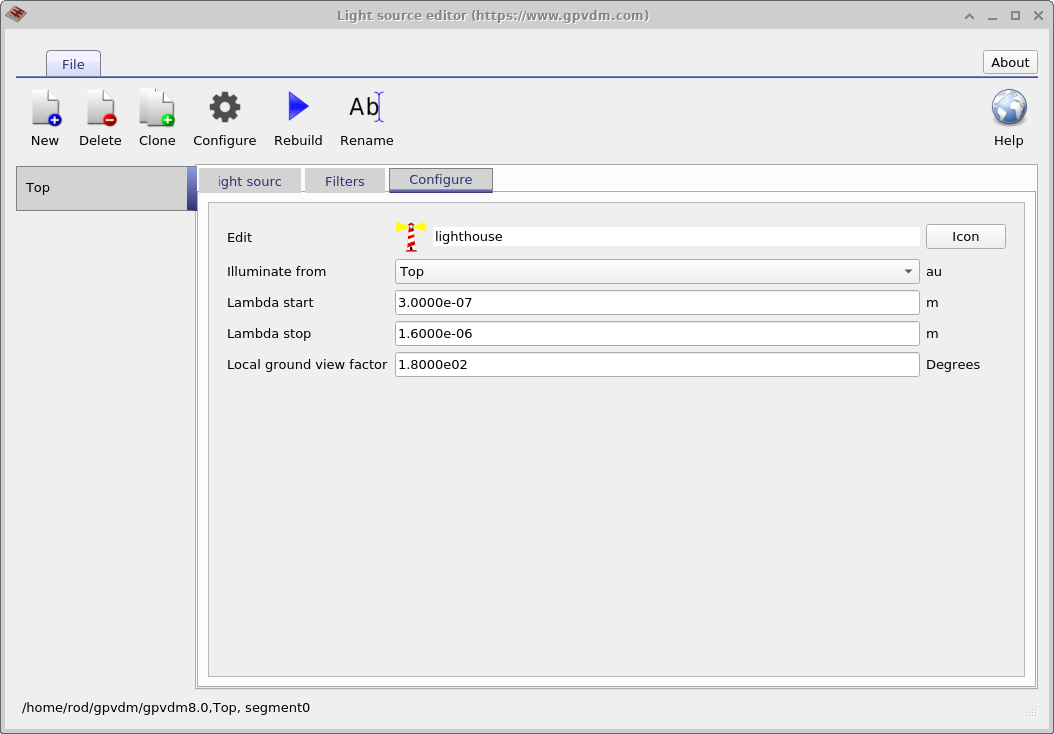
\includegraphics[width=0.5\textwidth,height=0.4\textwidth]{./images/lights2.png}

&
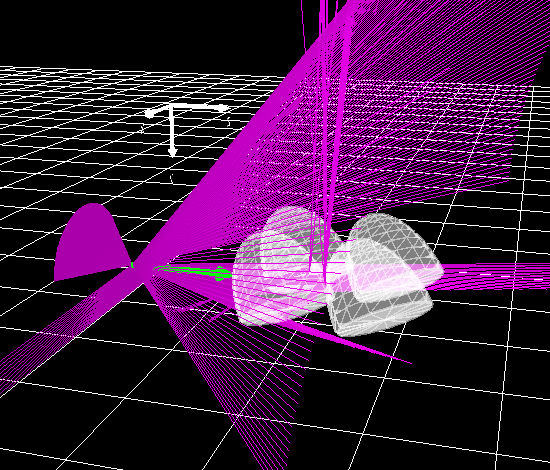
\includegraphics[width=0.5\textwidth,height=0.4\textwidth]{./images/light_xyz.png}
\\

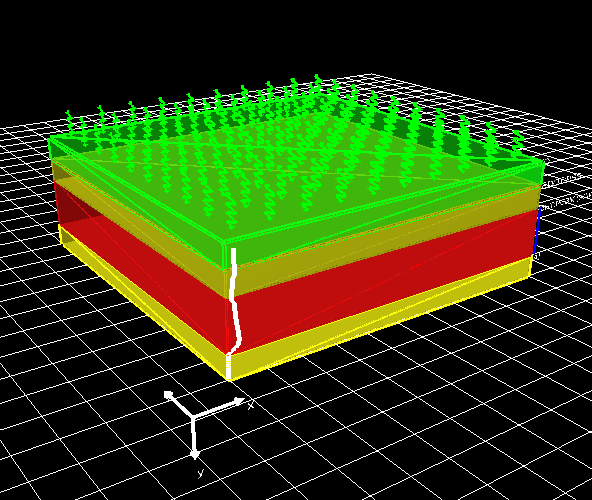
\includegraphics[width=0.5\textwidth,height=0.4\textwidth]{./images/light_top.png}

&
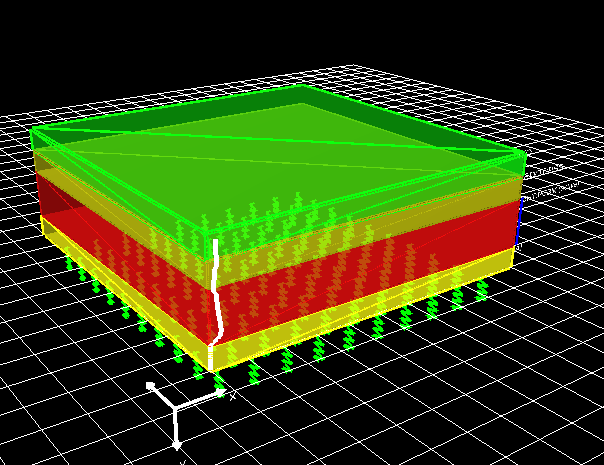
\includegraphics[width=0.5\textwidth,height=0.4\textwidth]{./images/light_btm.png}
\\
\end{tabular}
\caption{Top left: The configure panel of the light source editor; Top right: Illuminate from set to "xyz"; bottom left: Illuminate from set to "top"; bottom right: Illuminate from set to "bottom".}
\label{fig:lightcomesfrom}
\end{figure}





